\documentclass[a4paper,12pt]{article}
\pdfpagewidth\paperwidth
\pdfpageheight\paperheight
\usepackage[greek,italian]{babel}
\usepackage[utf8]{inputenc}
\usepackage[T1]{fontenc}
\usepackage{lmodern,amsmath,amssymb,tipa,cclicenses,geometry,graphicx,subcaption,apple_emoji,wasysym,tikz,dsfont,chemfig}
\usetikzlibrary{mindmap}
\usepackage[hidelinks]{hyperref}

\DeclareFontFamily{U}{min}{}
\DeclareFontShape{U}{min}{m}{n}{<-> dmjhira}{}
\newcommand{\se}[2]{\ensuremath{\textnormal{\usefont{U}{min}{m}{n}\char"1B}_{#1}^{#2}}}
\newcommand{\1}{\ensuremath{\mathds{1}}}
\newcommand{\Tikz}{Ti\emph{k}Z}

\DeclareUnicodeCharacter{2191}{$\uparrow$}

\begin{document}
\newgeometry{margin=25mm}
\title{Appunti per Corso introduttivo a \LaTeX}
\author{Davide Peressoni\\Aprile 2018}
\date{
\includegraphics[height=100px]{ComInfo}\\Commissione Informatica\\Collegio Universitario don Nicola Mazza}
\maketitle

\cc 2018 Davide Peressoni\\~\par
    \emph{Le informazioni contenute nel presente docuemnto sono state verificate e documentate con la massima cura possibile. Nessuna responsabilità derivante dal loro utilizzo potrà venire imputata all’Autore coinvolto nella loro creazione, pubblicazione e distribuzione.}\\~\par
    Alcuni diritti riservati.\\~\\
    Documento prodotto con \LaTeX.\\
    Questo documento è rilasciato con licenza\\
    \begin{figure}[!ht]
	\centering
	    
\includegraphics{../Lezione1/CC.pdf}
    \end{figure}~\\
    \textbf{Creative Commons BY-NC-SA 4.0}\\
    Attribuzione – Non Commerciale - Stessa licenza\\
    \url{http://creativecommons.org/licenses/by-nc-sa/4.0/}\\
    \textbf{Attribuzione} — Devi riconoscere una menzione di paternità adeguata, fornire un link alla licenza e indicare se sono state effettuate delle modifiche. Puoi
    fare ciò in qualsiasi maniera ragionevole possibile, ma non con modalità tali da suggerire che il licenziante avalli te o il tuo utilizzo del materiale.\\
    \textbf{Non commerciale} — Non puoi usare il materiale per scopi commerciali.\\
    \textbf{Stessa licenza} — Se remixi, trasformi il materiale o ti basi su di esso, devi distribuire i tuoi contributi con la stessa licenza del materiale originario.
\restoregeometry\newpage
\tableofcontents
\addcontentsline{toc}{section}{Indice} %aggiunge voce indice nell'indice
\label{contents}    %dice dove si torva l'indice per il punto sopra
\newpage

\section{Cos'\`{e} \LaTeX?}
  \LaTeX{} è un linguaggio di markup che ci permette di descrivere il documento. A differenza dei più famosi editor (come Writer, Word, Google Docs, ...) non vediamo il risultato mentre scriviamo, ma solo dopo aver \emph{compilato} il documento.
  \begin{figure}[!h]
    \centering
    \begin{subfigure}[b]{0.4\textwidth}
        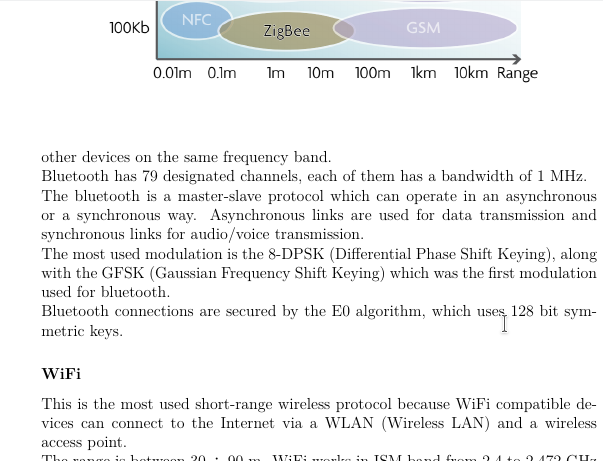
\includegraphics[width=\textwidth]{img/writer}
        \caption{Writer}
    \end{subfigure}~
    \begin{subfigure}[b]{0.4\textwidth}
        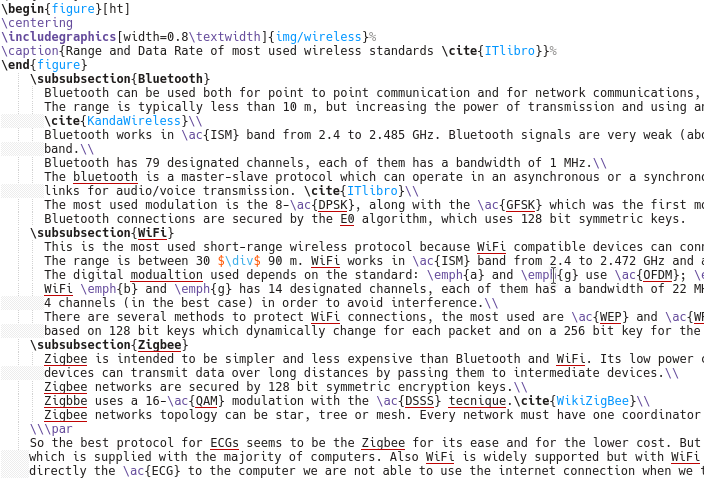
\includegraphics[width=\textwidth]{img/latex_source}
        \caption{Latex}
    \end{subfigure}
  \end{figure}
  \subsection{I vantaggi di \LaTeX}
\begin{itemize}
\item I documenti hanno un'impaginazione perfetta e risultano piacevoli alla lettura
\item Con un po' di esercizio di possono comporre formule matematiche, schemi a blocchi, circuiti,\dots{} semplicemente
\item La formattazione non subirà mai modifiche drastiche e risulterà uniforme
\end{itemize}
\newpage
\subsection{Cosa si può fare con \LaTeX?}
\begin{figure}[!h]\centering
  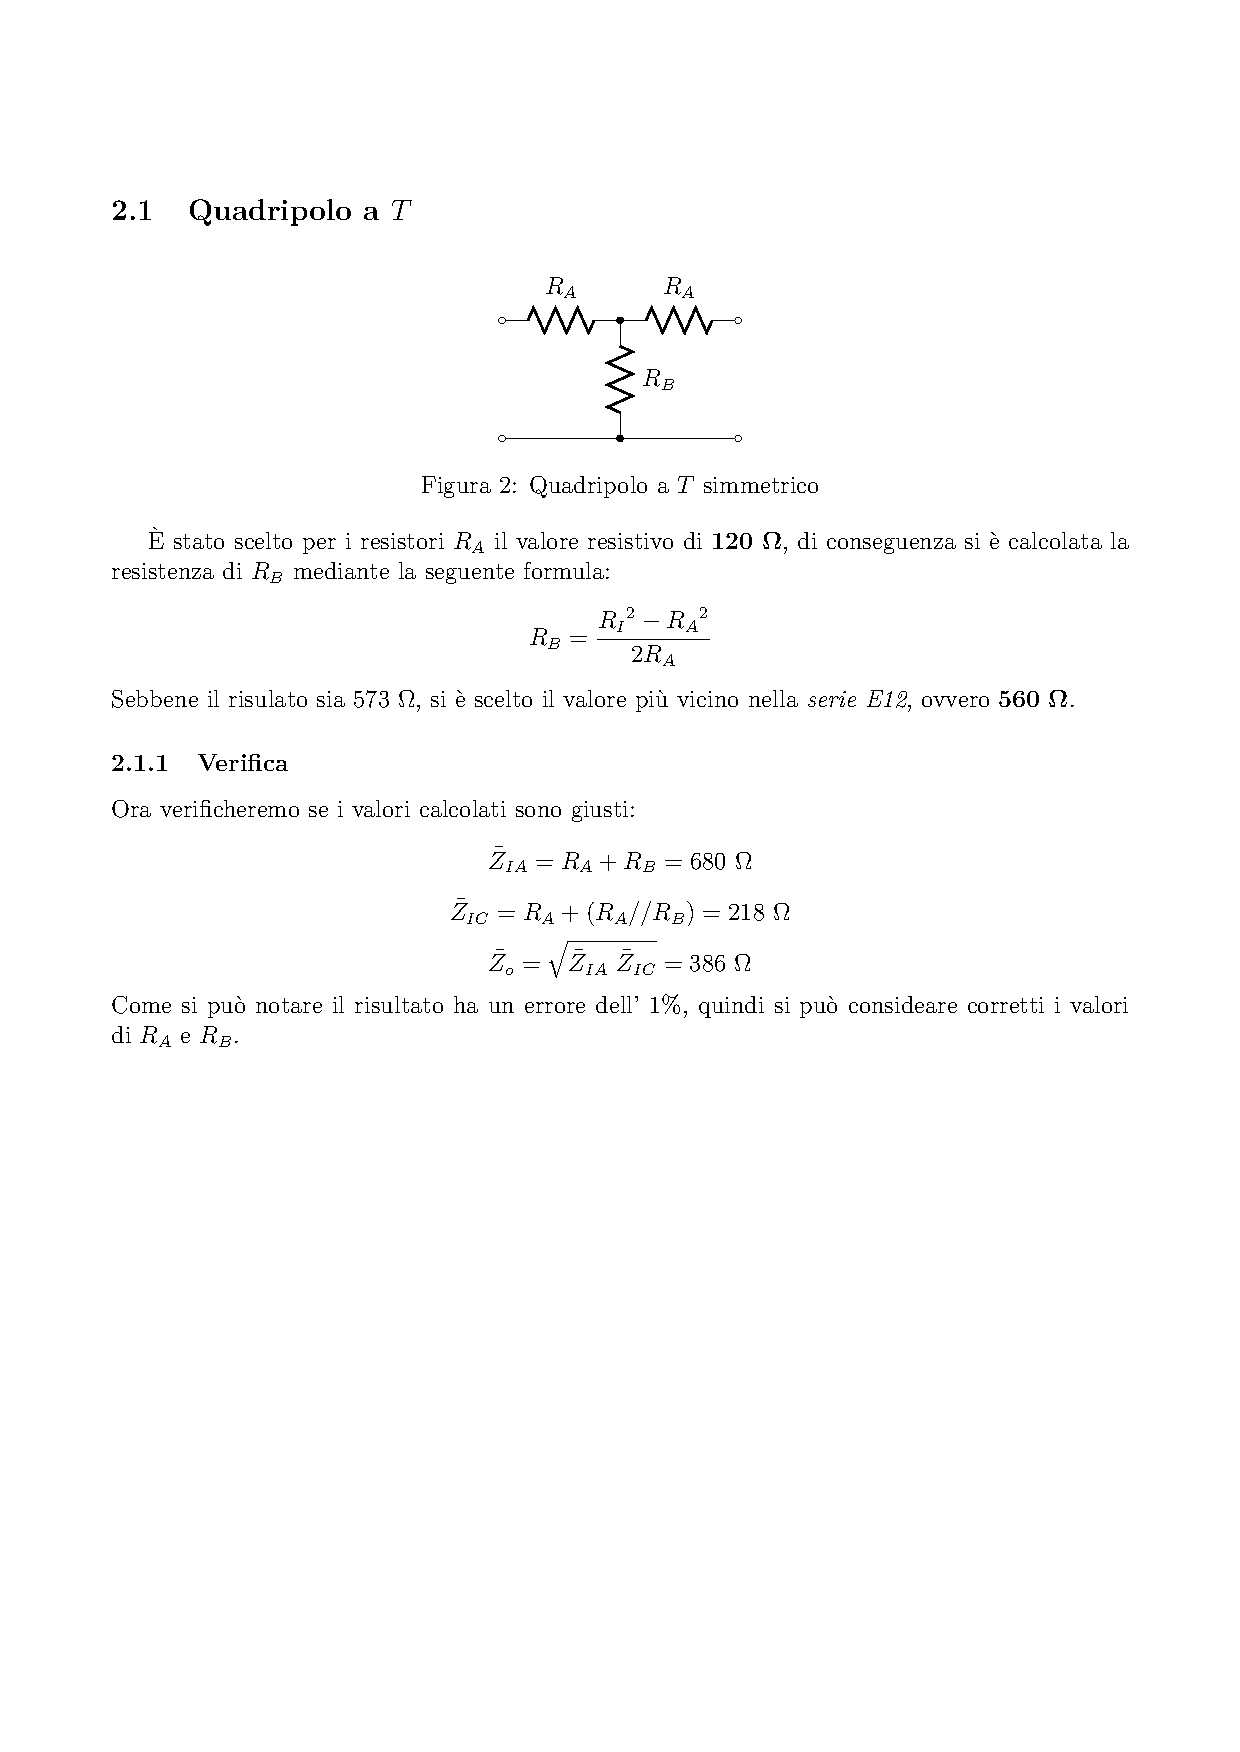
\includegraphics[trim={0 0 0 5.2cm},clip,width=0.9\textwidth]{img/relazione}
  \caption{Articoli, Relazioni, Libri, Lettere,~\dots}
\end{figure}
\begin{figure}[!h]\centering
  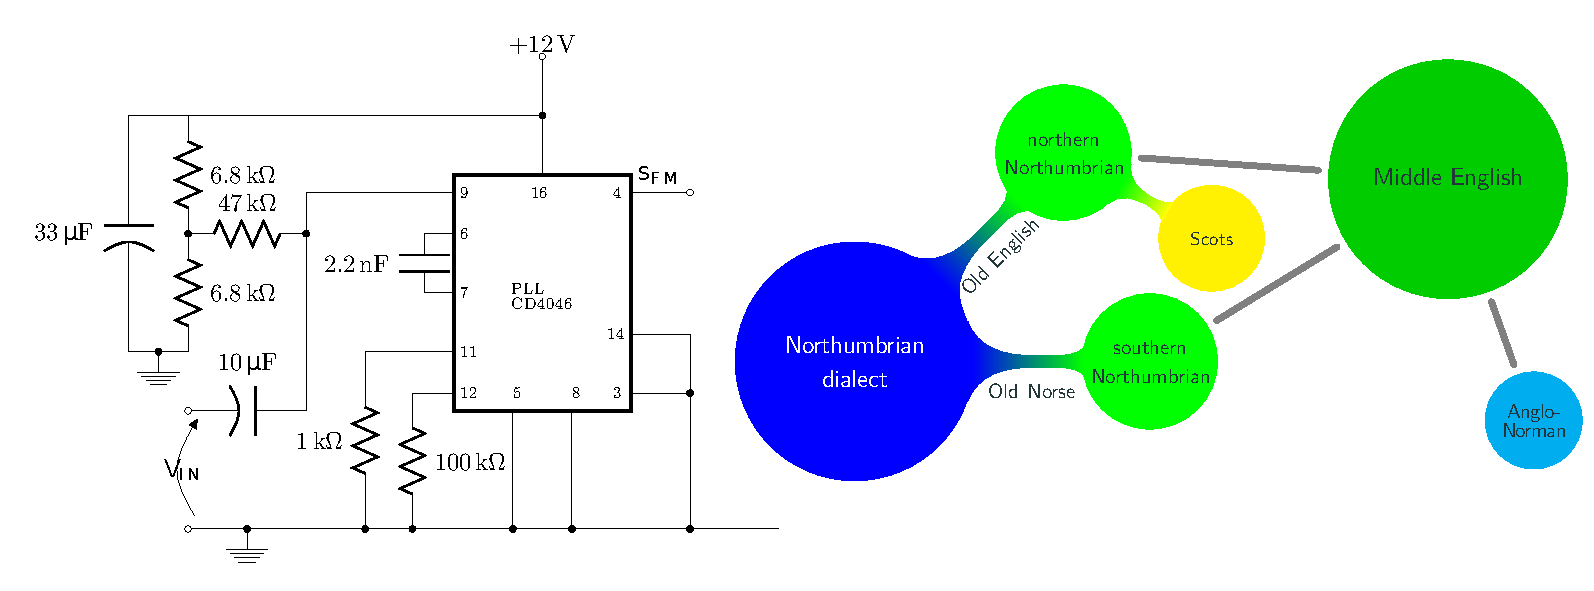
\includegraphics[width=0.9\textwidth]{img/schemi}
  \caption{Circuiti, Schemi, Tabelle, Grafici,~\dots}
\end{figure}
\newpage\vspace{100px}
\begin{figure}[!h]\centering
  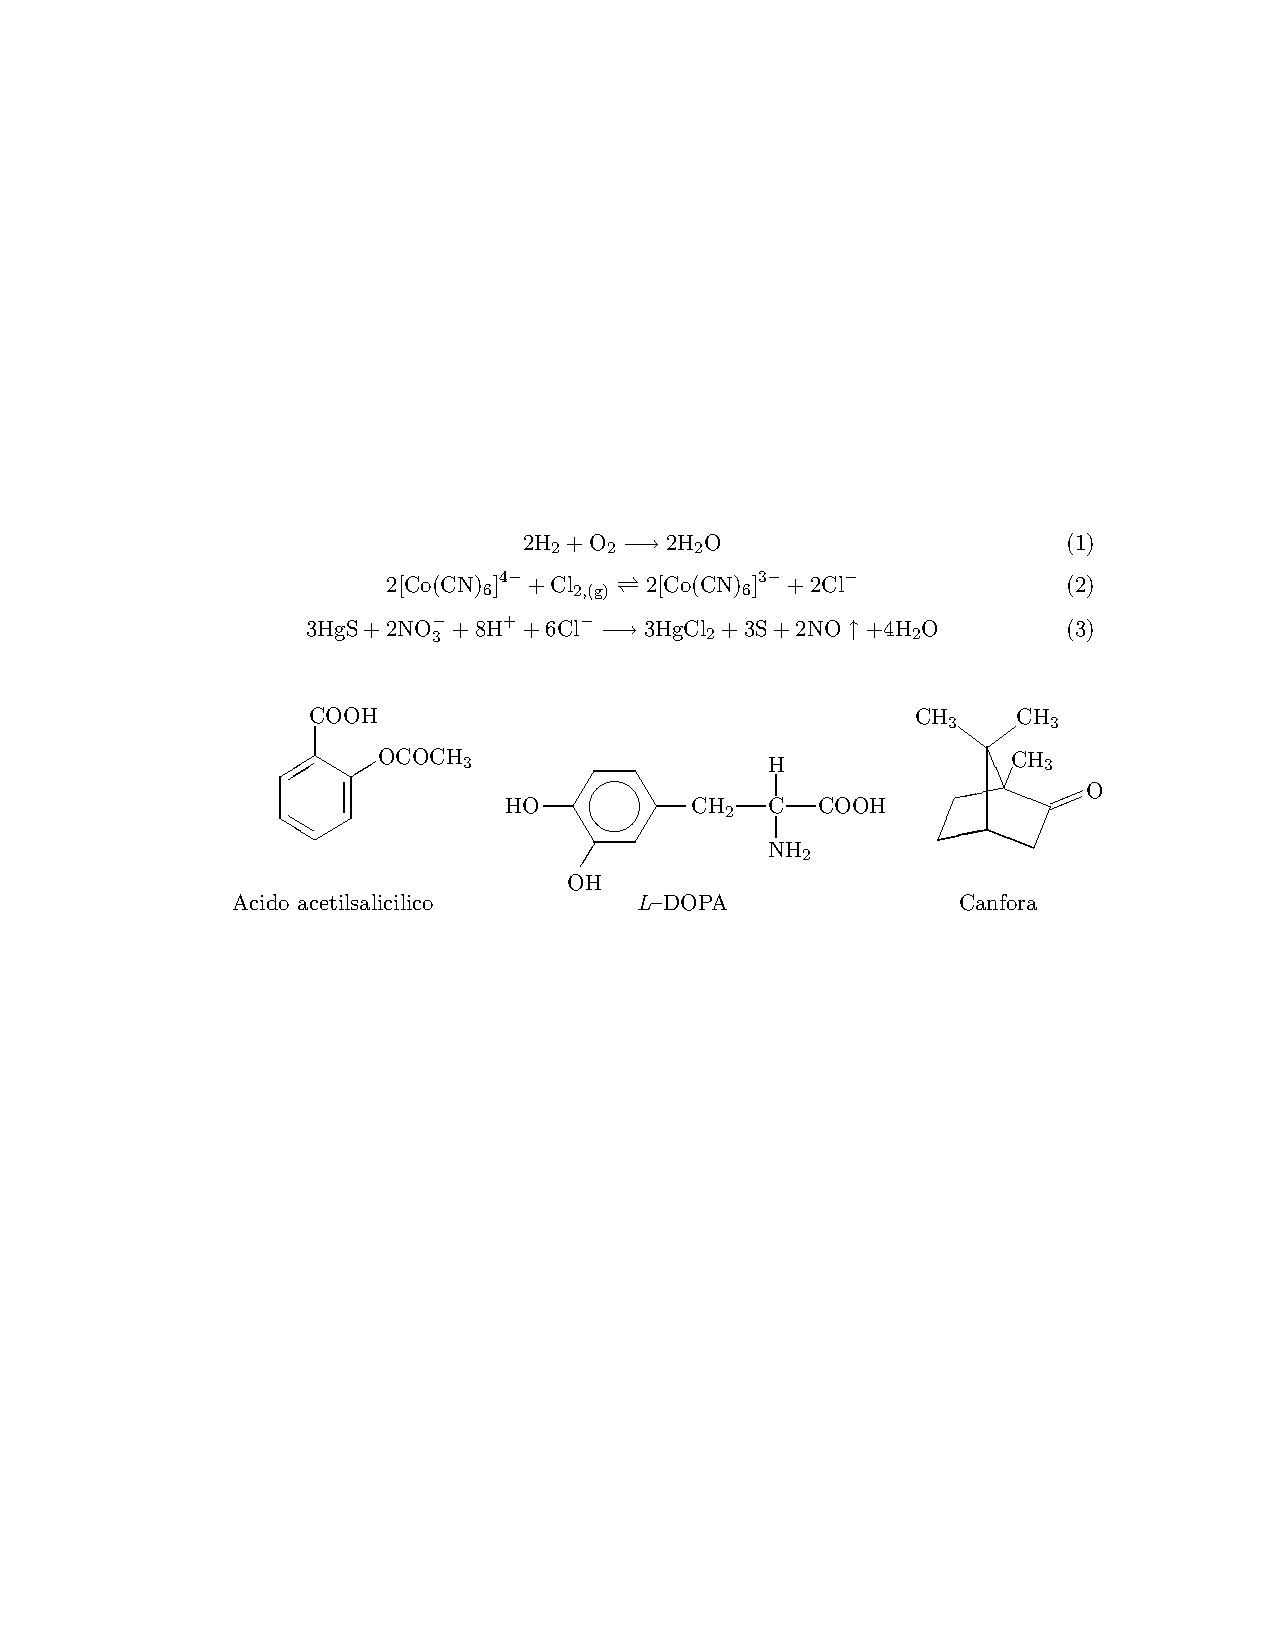
\includegraphics[width=0.9\textwidth]{img/chimica}
  \caption{Formule chimiche}
\end{figure}\vspace{100px}
\begin{figure}[!h]
  \captionsetup[subfigure]{labelformat=empty}
    \centering
    \begin{subfigure}[b]{0.4\textwidth}
        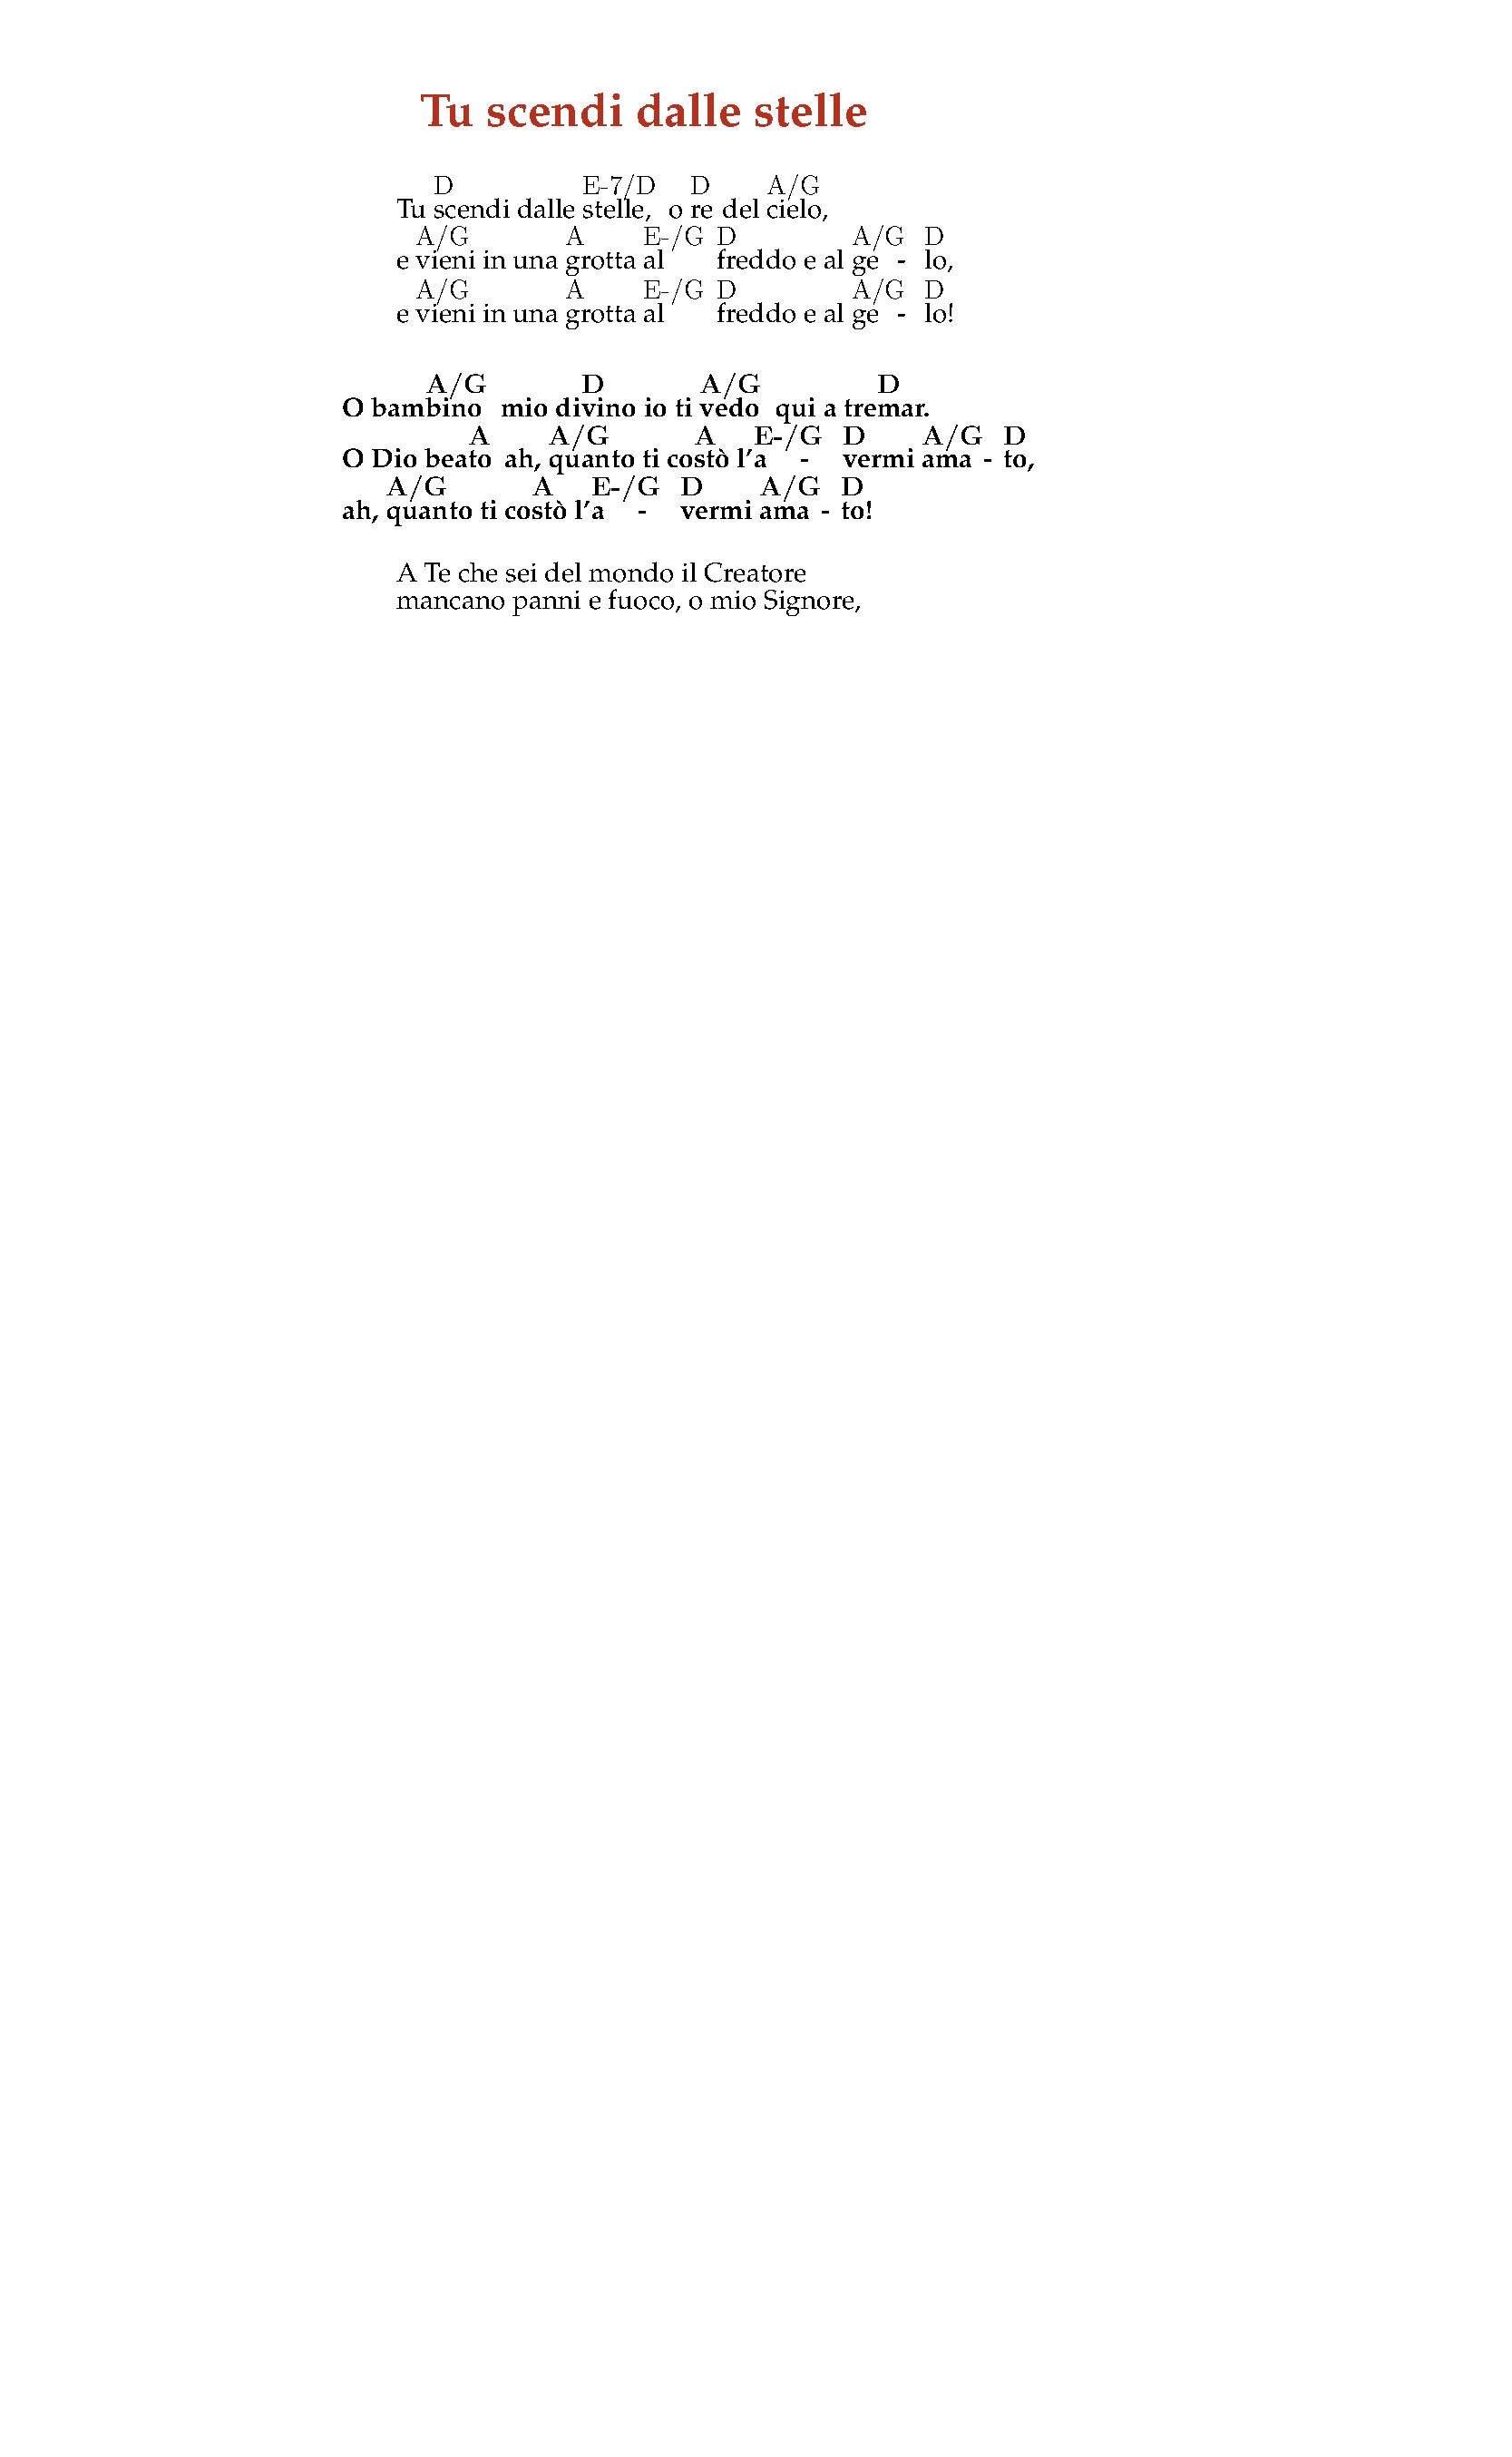
\includegraphics[width=\textwidth]{img/accordi}
    \end{subfigure}~
    \begin{subfigure}[b]{0.6\textwidth}
        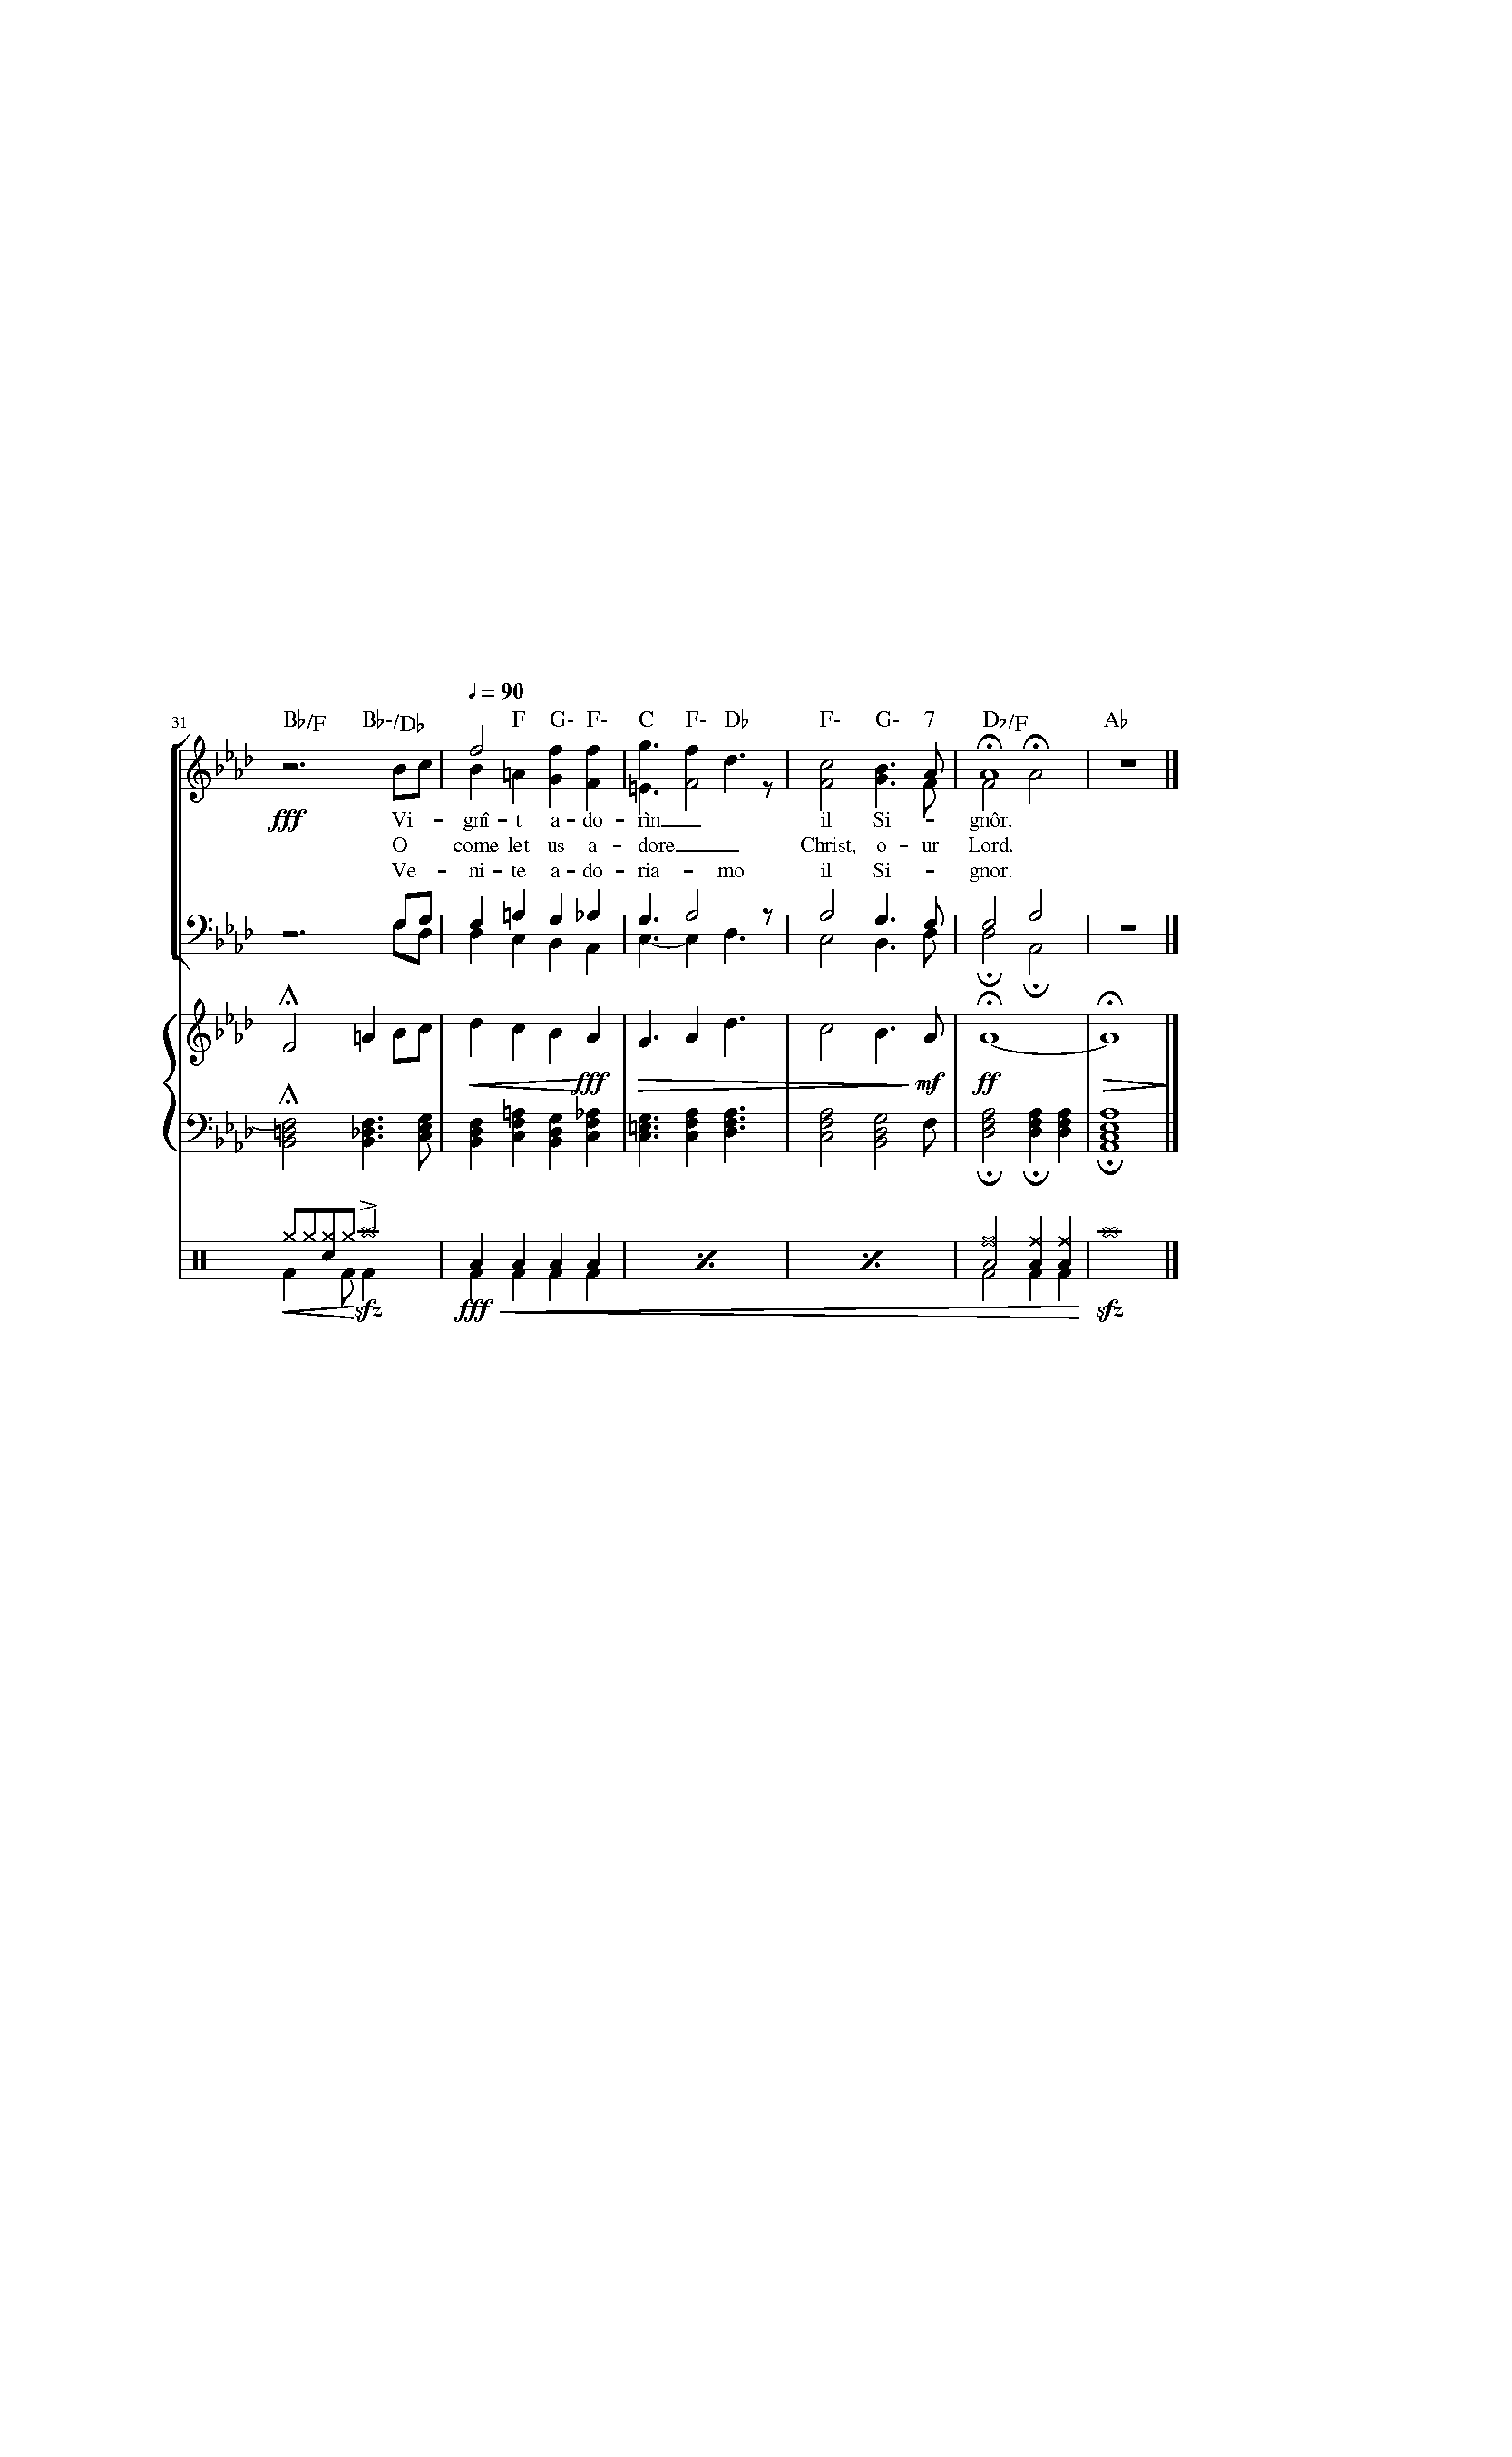
\includegraphics[width=\textwidth]{img/spartiti}
    \end{subfigure}
  \caption{Accordi, Spartiti,~\dots}
\end{figure}\vspace{100px}\newpage
\begin{figure}[!h]\centering
  
\includegraphics[width=0.7\textwidth,page=1]{img/presentazione}
  \caption{Presentazioni}
\end{figure}
\begin{figure}[!h]\centering
  
\includegraphics[width=\textwidth,page=1]{img/alfabeti}
  \caption{Scrivere con più alfabeti}
\end{figure}
\subsection{Come si utilizza \LaTeX?}
  Per scrivere un docuemnto con \LaTeX si può usare un qualsiasi editor di testo piano (Notepad++, Kate, gedit, VScode, Atom, vi, vim, nano, \dots) e un compilatore a linea di comando (come pdflatex).\\
  Per facilitare le cose si può usare degli editor avanzati come Miktex, i quali non richiedono l'uso della linea di comando e forniscono un buon supporto alla scrittura del documento.

\section{Tipologie di documento}
  \begin{itemize}
    \item \textbf{\emph{article}} per scrivere articoli (scientifici) senza capitoli
    \item \textbf{report} per scrivere relazioni o tesi suddivise in capitoli
    \item \textbf{letter} per scrivere lettere
    \item \textbf{\emph{book}} per scrivere libri
    \item {\footnotesize\textbf{memoir} per scrivere libri complessi}
    \item {\footnotesize\textbf{beamer} per presentazioni}
    \item \textbf{\dots}
  \end{itemize}

\section{Esempio minimale}
\begin{verbatim}
  \documentclass[a4paper, twocolumn, 12pt]{report}
    %               10pt, 11pt, 12 pt ↑       ↑ classe
    %    twocolumn dispone il testo su due colonne

  \pdfpagewidth\paperwidth      % per assicurarsi che nel pdf
  \pdfpageheight\paperheight    % sia riempita tutta la pagina

  \usepackage[italian]{babel}   % lingua usata nel documento
  \usepackage[utf8]{inputenc}  % se non va usare utf8x o alla peggio latin1
  \usepackage[T1]{fontenc}

  \begin{document}
    \title{Titolo del documento}\author{Autore}\date{Data}
    \maketitle

    \tableofcontents  %indice

    \chapter{Nome capitolo}
      testo
      \section{Nome sezione}
        testo
        \subsection{Nome sottosezione}
          testo
          \subsubsection{Nome sotto-sottosezione}
            testo

  \end{document}
  \end{verbatim}

  \subsection{Andare a capo}
  \begin{itemize}
    \item{\texttt{\textbf{\textbackslash\textbackslash}} a capo}
    \item{\texttt{\textbf{\textbackslash par}} nuovo paragrafo}
  \end{itemize}
\subsection{Alcuni simboli}
  \begin{itemize}
    \item{\texttt{\textbf{\textbackslash\$}} \$}
    \item{\texttt{\textbf{\textbackslash\%}} \%}
    \item{\texttt{\textbf{\textbackslash\_}} \_}
  \end{itemize}
  In genere tutti i simboli che hanno un significato in \LaTeX{} (vedremo che avrenno questo ruolo \&, \$, \^{}, \_, \dots) si scrivono come sopra.

\section{Font}
  \subsection{Stili principali}
  \begin{itemize}
    \item{\texttt{\textbf{\textbackslash textbf}}\{testo\} \textbf{grassetto}}
    \item{\texttt{\textbf{\textbackslash emph}}\{testo\} \emph{italico} ("corsivo")}
    \item{\texttt{\textbf{\textbackslash texttt}}\{testo\} \texttt{monospace}}
  \end{itemize}
  \subsection{Dimensioni principali}
  \begin{itemize}
    \item{\{\texttt{\textbf{\textbackslash tiny}} \tiny testo \}}
    \item{\{\texttt{\textbf{\textbackslash footnotesize}} \footnotesize testo \}}
    \item{\{\texttt{\textbf{\textbackslash small}} \small testo \}}
    \item{\{\texttt{\textbf{\textbackslash large}} \large testo \}}
    \item{\{\texttt{\textbf{\textbackslash Large}} \Large testo \}}
  \end{itemize}

\section{Matematica}
Per le formule matemtiche e per altri simboli occorre includere i seguenti pacchetti (nel preambolo):
\verb!\usepackage{amsmath,amssymb}!
\subsection{Formule in linea}
  \texttt{Come tutti sanno \textbf{\$2\^{}2 = 4\$} e \textbf{\$2 \textbackslash times 2 = 4\$}}\\
  Come tutti sanno $2^2 = 4$ e $2 \times 2= 4$
\subsection{Formule in evidenza}
  \texttt{Data la funzione: \textbf{\textbackslash[ f(x)= x\^{}2 + \textbackslash frac\{x\}\{2\} \textbackslash]}}\\~\\
  Data la funzione: \[ f(x)= x^2 + \frac{x}{2} \]
\subsection{Formule in evidenza numerate}
  \texttt{Data la funzione: \textbf{\textbackslash begin\{equation\} f(x):= x\^{}2 + \textbackslash frac\{x\}\{2\} \\ \textbackslash label\{eq:\emph{nomeFormula}\} \textbackslash end\{equation\}}}\\~\\
Data la funzione: \begin{equation} f(x):= x^2 + \frac{x}{2} \label{eq:nomeFormula}\end{equation}
  \texttt{Vedi formula \textbf{\textbackslash ref\{eq:\emph{nomeFormula}\}}}\\~\\
Vedi formula \ref{eq:nomeFormula}\\
Perché il numero compaia giusto bisogna compilare 2 volte.
\subsection{Esempi}
\verb!\forall x \in X, \quad \exists y \leq \epsilon!\[\forall x \in X, \quad \exists y \leq \epsilon\]
  \verb!\cos (2\theta) = \cos^2 \theta - \sin^2 \theta!\[\cos (2\theta) = \cos^2 \theta - \sin^2 \theta\]
  \verb!\lim_{x \to \infty} \exp(-x) = 0! \[
  \lim_{x \to \infty} \exp(-x) = 0\]
  \verb!x \equiv a \pmod{b}! \[x \equiv a \pmod{b}\]
  \verb!k_{n+1} = n^2 + k_n^2 - k_{n-1}!\[k_{n+1} = n^2 + k_n^2 - k_{n-1}\]
  \verb!\sqrt{2} \sqrt[n]{\frac{a}{b}}! \[\sqrt2 ~~~~ \sqrt[n]{\frac{a}{b}}\]
  \verb!\sum_{i=1}^{10} t_i! \[\sum_{i=1}^{10} t_i\]
  \verb!\displaystyle\sum_{i=1}^{10} t_i! \[\displaystyle\sum_{i=1}^{10} t_i\]
  \verb!\int_0^\infty \mathrm{e}^{-x}\,\mathrm{d}x! \[\int_0^\infty \mathrm{e}^{-x}\,\mathrm{d}x\]
  \verb!A_{2,2} = \begin{pmatrix}         !\\
  \verb!              a_{1,1} & a_{1,2} \\!\\
  \verb!              a_{2,1} & a_{2,2}   !\\
  \verb!          \end{pmatrix}           !\\~\\
    \[A_{2,2} = \begin{pmatrix}a_{1,1} & a_{1,2} \\a_{2,1} & a_{2,2}\end{pmatrix}\]

\section{Elenchi}
\subsection{Elenchi numerati}
  \verb!\begin{enumerate}!\\
  \verb!  \item Tizio     !\\
  \verb!  \item Caio      !\\
  \verb!  \item Sempronio!\\
  \verb!\end{enumerate}  !\\~
  \begin{enumerate}
    \item Tizio
    \item Caio
    \item Sempronio
  \end{enumerate}
\subsection{Elenchi puntati}
  \verb!\begin{itemize}   !\\
  \verb!  \item Tizio     !\\
  \verb!  \item Caio      !\\
  \verb!  \item Sempronio!\\
  \verb!\end{itemize}     !\\~
  \begin{itemize}
    \item Tizio
    \item Caio
    \item Sempronio
  \end{itemize}
  \verb!\begin{itemize}   !\\
    \verb!  \item[-] Tizio     !\\
    \verb!  \item[$x^2$] Caio      !\\
    \verb!  \item[$\star$] Sempronio!\\
    \verb!\end{itemize}     !\\~
    \begin{itemize}
      \item[-] Tizio
      \item[$x^2$] Caio
      \item[$\star$] Sempronio
    \end{itemize}
\subsection{Descrizioni}
  \verb!\begin{description}              !\\
  \verb!  \item[Responsabile] Tizio      !\\
  \verb!  \item[Supervisore] Caio        !\\
  \verb!  \item[Collaboratore] Sempronio!\\
  \verb!\end{description}                !\\~
  \begin{description}
    \item[Responsabile] Tizio
    \item[Supervisore] Caio
    \item[Collaboratore] Sempronio
  \end{description}

\section{Note}
\subsection{Note a piè di pagina}
  \verb!Questo è un testo\footnote{è un testo molto corto} di prova!\\~\\
  Questo è un testo\footnote{è un testo molto corto} di prova
\subsection{Note al margine}
  \texttt{L'area\textbackslash marginpar\{\$A = l\^{}2\$\} del quadrato vale 5}\\~\\
   L'area\marginpar{$A = l^2$} del quadrato vale 5

\section{Problemi di numeri di pagina}
	Se usiamo la classe \emph{book} notiamo che i numeri di pagina della prima pagina di un capitolo rimangono in basso.\\
	Per ovviare questo problema inserite nel preambolo (prima del \textbackslash begin\{document\}):\\
	\texttt{\textbackslash newcommand\{\textbackslash hchapter\}[1]\{\textbackslash newpage\textbackslash pagestyle\{empty\}\\              \textbackslash chapter\{\#1\}\textbackslash thispagestyle\{headings\}\textbackslash pagestyle\{headings\}\}}\par
	E usate \texttt{\textbackslash \textbf{h}chapter} anzi che \verb!\chapter!.\par
	Questi purtroppo non risolvono il problema nell'indice e qui consiglio di scrivere:\\
	\verb!\tableofcontents\thispagestyle{plain}!~\par
	Se invece non volete il numero di pagina nei nuovi capitoli (che è forse più elegante): \\
	\texttt{\textbackslash newcommand\{\textbackslash hchapter\}[1]\{\textbackslash newpage\textbackslash pagestyle\{empty\}\\              \textbackslash chapter\{\#1\}\textbackslash thispagestyle\{empty\}\textbackslash pagestyle\{headings\}\}}


\section{Tabelle}
  \verb!\begin{tabular}{lc|r}                   !\\
  \verb!  Nome        & Cognome & Età \\ \hline !\\
  \verb!  Pinco Tizio & Pallino & 6 \\          !\\
  \verb!  Mario       & Rossi   & 23            !\\
  \verb!\end{tabular}                           !\\~\\
    \begin{tabular}{lc|r}
      Nome & Cognome & Età \\ \hline
      Pinco Tizio & Pallino & 6 \\
      Mario & Rossi & 23
    \end{tabular}\\
~\\~
    \\\verb!\begin{table}                       !\\
    \\\verb!\centering %allinea la tabella al centro!\\
    \verb!  \begin{tabular} ... \end{tabular} !\\
    \verb!  \caption{Utenti del servizio}     !\\
    \verb!  \label{tab:Utenti}                !\\
    \verb!\end{table}                         !\\
      \begin{table}[!h]\centering
        \begin{tabular}{lc|r}
          Nome & Cognome & Età \\ \hline
          Pinco Tizio & Pallino & 6 \\
          Mario & Rossi & 23
        \end{tabular}
        \caption{Utenti del servizio}
        \label{tab:Utenti}
      \end{table}
      ~\\~\texttt{come si evince dalla tabella \textbackslash ref\{tab:Utenti\} \textbackslash dots} \\Come si evince dalla tabella \ref{tab:Utenti} \dots

\section{Immagini}
 \subsection{Immagini in linea}
  \texttt{\textbackslash usepackage\{graphicx\} \% da inserire prima dell'inizio del docuemnto}\\
  \texttt{\textbackslash includegraphics\{disegno\}}\\~\\
  
\includegraphics[height=100px]{img/disegno}\\
  \texttt{\textbackslash includegraphics[width=300px,height=50px]\{disegno\}}\\~\\
  
\includegraphics[width=300px,height=50px]{img/disegno}~\\~
  \texttt{\textbackslash includegraphics[width=\textbackslash textwidth]\{disegno\}}\\~\\
  
\includegraphics[width=\textwidth]{img/disegno}~\\~
  Come argomento va inserito il nome del file senza estensione. Sono supportate immagini PDF, PNG e JPEG.\\
  Questo tipo di insierimento si dice in linea perché l'immagine "fa parte" del testo:\\
  \texttt{Questa è \textbackslash includegraphics\{disegno\} una prova}\\~\\
  Questa è 
\includegraphics[height=100px]{img/disegno} una prova\par
  Alcune librerie (come apple\_emoji) permettono di inserire emoji nel testo proprio sfruttando questo sistema.\\
  \verb!\usepackage{apple_emoji}!\\
  \texttt{Ciao \smiley, come va?} $\Rightarrow$ Ciao 😀, come va?
  \subsection{Immagini come figure}
  \verb!\begin{figure}                       !\\
	\\\verb!\centering %allinea l'immagine' al centro!\\
  \verb!  \includegraphics{immagine}         !\\
  \verb!  \caption{Disegno astratto}         !\\
  \verb!  \abel{fig:Disegno}                 !\\
  \verb!\end{figure}                         !\\
  \begin{figure}[!ht]\centering%
    
\includegraphics[height=60px]{img/disegno}%
    \caption{Disegno astratto}%
    \label{fig:Disegno}%
  \end{figure}\\%
  \texttt{Visibile in figura \textbackslash ref\{fig:Disegno\}} $\Rightarrow$ Visibile in figura \ref{fig:Disegno}

\section{Riferimenti}
  \texttt{Nel bel mezzo del cammin di nostra vita\textbackslash label\{sec:Prologo\}}\label{sec:Prologo}\\~\\
  \texttt{Come si legge nella sezione \textbackslash ref\{sec:Prologo\} a pagina \textbackslash pageref\{sec:Prologo\}}\\
 Come si legge nella sezione \ref{sec:Prologo} a pagina \pageref{sec:Prologo}
 \begin{table}[!ht]\centering
 \begin{tabular}{l|l}
  prefisso & ambiente\\\hline
  ch: 	&chapter\\
  sec: 	&section\\
  subsec: 	&subsection\\
  fig: 	&figure\\
  tab: 	&table\\
  eq: 	&equation\\
\end{tabular}\end{table}
\\Se si vuole che nel pdf risualtante i riferimenti siano cliccabili (come dei link) bisogna aggiungere nel preambolo: \verb!\usepackage[hidelinks]{hyperref}! (se non si mette [hidelinks] i link saranno circondati di un colore che li contraddistingue in base al tipo di referenze secondo alcuni standard,
\hypersetup{pdfborder={0 0 0.5}}
 esempio: nella sezione \ref{sec:Prologo}
\hypersetup{hidelinks})

\section{Bibliografia}
\verb!\begin{thebibliography}{Numero massimo voci} !\\
  \verb!  \addcontentsline{toc}{section}{Bibliografia} !\\
  \verb!  \label{bibliografia} !\\
  ~\\
  \verb!  \bibitem{WiFiStandard} %etichetta!\\
  \verb!    Ian Poole,\\ !\\
  \verb!    \emph{IEEE 802.11 Wi-Fi Standards},\\ !\\
  \verb!    \url{http://www.radio-electronics.com/info/wireless/wi-fi/!\\
  \verb!         ieee-802-11-standards-tutorial.php},\\ !\\
  \verb!    consultato il 3 Giugno 2017. !\\
  ~\\
  \verb! \end{thebibliography} !\\~\par
  Il numero massimo di voci serve all'allineamento dei numeri, è consigliato scrivere tanti 8 quante le cifre del numero più grande (ad esempio se avete 15 libri in bibliografia scrivete 88).

      \begin{thebibliography}{8}
        \bibitem{WiFiStandard}
          Ian Poole,\\
          \emph{IEEE 802.11 Wi-Fi Standards},\\
          \url{http://www.radio-electronics.com/info/wireless/wi-fi/ieee-802-11-standards-tutorial.php},\\
          consultato il 3 Giugno 2017.
      \end{thebibliography}
\subsection{Richiamo della bibliografia}
\texttt{... che utilizza modulazioni digitali \textbackslash cite\{WiFiStandard\}}~\\~
... che utilizza modulazioni digitali~\cite{WiFiStandard}\\~


\section{Inserire simboli}
\subsection{Siti}
  \begin{itemize}
    \item Simboli matematici\\
      \url{https://en.wikibooks.org/wiki/LaTeX/Mathematics}
    \item Tutti(?) i simboli\\
      \url{http://tug.ctan.org/info/symbols/comprehensive/symbols-a4.pdf}
  \end{itemize}
\subsection{Detextify}
  \url{http://detexify.kirelabs.org}
  ~\\~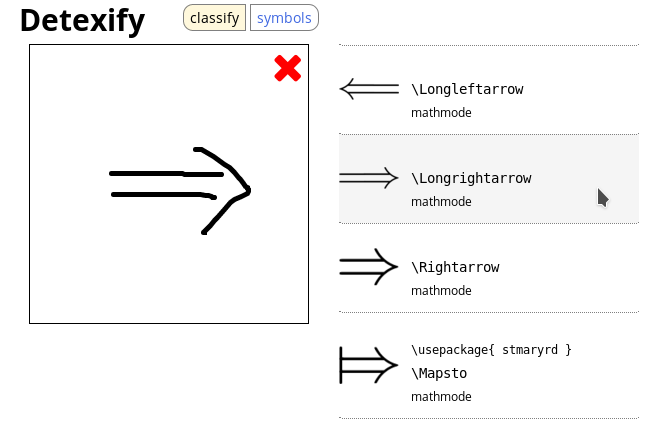
\includegraphics[width=\textwidth]{img/detex}~\\~
  Ti permette di disegnare il simbolo e ti mostra il comando per inserirlo, l'ambiente (testo o matematico) ed eventuali pacchetti da importare.
  
  
\section{Scrivere in greco}
Nel preambolo: \verb!\usepackage[greek,italian]{babel}!\\
Nel documento: \\
\verb!\TeX~deriva dal greco \begin{otherlanguage}{greek}t'eqnh!\\
\verb!\end{otherlanguage}~(arte, tecnica)!\\
\TeX~deriva dal greco \begin{otherlanguage}{greek}t'eqnh\end{otherlanguage}~(arte, tecnica)

\section{Presentazioni}
  \texttt{\textbackslash{}documentclass[aspectratio=169]\{beamer\} \% prima riga} 
  \texttt{\\\dots\\
  \textbackslash{}begin\{frame\} \%dentro il document
\\
  ~~\textbackslash{}frametitle\{Titolo\}~~~~~~~~~~~~~
\\
  ~~\textbackslash{}framesubtitle\{Sottotitolo\}~~~~~
\\
  \textbackslash{}end\{frame\}
~~~~~~~~~~~~~~~~~~~~~~~\\~}
  \subsection{Comandi noti}
  Titolo: \texttt{\textbackslash{}maketitle}\\~\\
  \texttt{\textbackslash{}section, \textbackslash{}subsection}\\~\\
  Formattazione testo, immagini, note a piè di pagina, bibliografia, \dots

  \subsection{Indice}
  \texttt{~\\
  \textbackslash{}begin\{frame\}~~~~~~~~~~~\\
  ~~\textbackslash{}frametitle\{Contenuti\}\\
  ~~\textbackslash{}tableofcontents~~~~~~~~\\
  \textbackslash{}end\{frame\}~~~~~~~~~~~~~\\~
}
\subsection{Animazioni}
  \texttt{Questa è \textbackslash{}pause una prova}
\subsection{Temi e colori}
  \begin{tabular}{ll}
    \texttt{\textbackslash{}usetheme\{Warsaw\}}& Esempi di tutte le combinazioni tema-colore:\\
    \texttt{\textbackslash{}usecolortheme\{seahorse\}} & \url{https://hartwork.org/beamer-theme-matrix/}
  \end{tabular}
  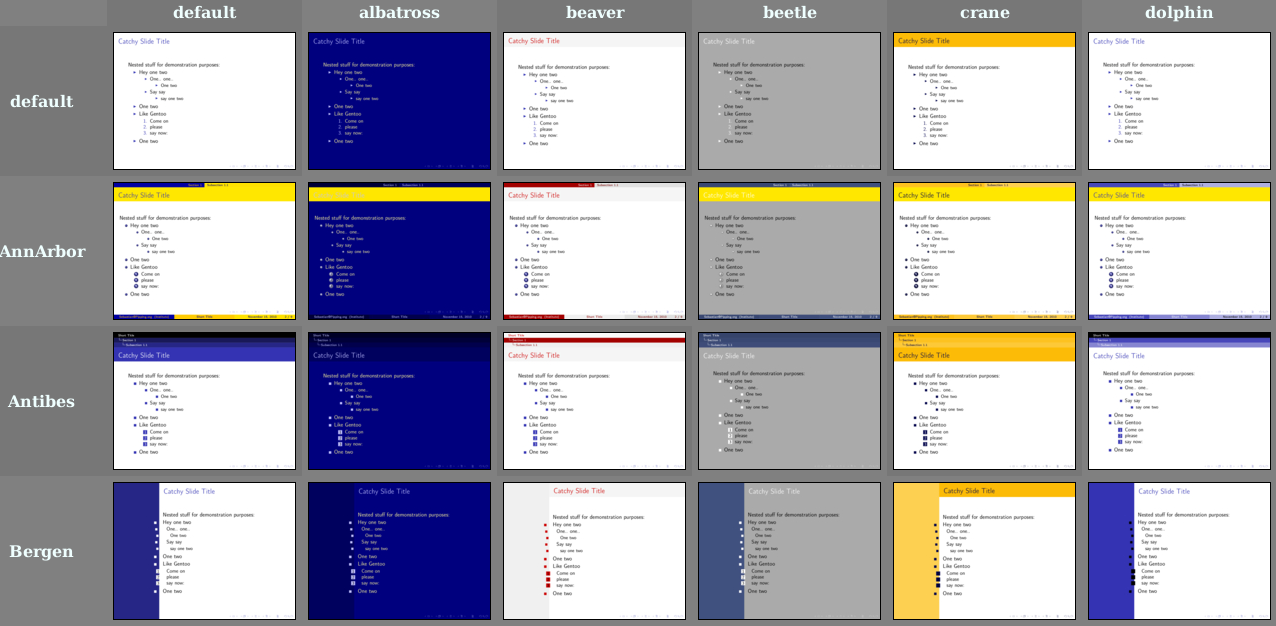
\includegraphics[width=\textwidth]{img/beamer}

\section{\Tikz}
  Libreria grafica per disegnare (descrivere disegni) con LaTeX.\\
  Offre un piano cartesiano su cui disegnare mediante dei comandi.\\~\\
  \texttt{\textbackslash{}usepackage\{tikz\} \%preambolo}\\
  \dots\\\texttt{
  \textbackslash{}begin\{tikzpicture\}\\
  \dots\\
  \textbackslash{}end\{tikzpicture\}~~\\~}
\subsection{Disegnare}
\subsubsection{Punti}
  \texttt{(1cm,2pt)} è un punto a coordinata x 1cm dall'origne e y 2pt dall'origine\\~\\
  \texttt{(30:1cm)} è un punto sulla circonferenza di raggio 1 cm, a 30 gradi (coordinate polari)\\~\\
  \texttt{++(1cm,2cm)} le coordinate sono relative a quelle del punto precedente e non all'origine\\~\\
  \texttt{+(1cm,2cm)} come \texttt{++} ma non aggiorna le coordinate dell'ultimo punto
\subsubsection{path}
  \texttt{\textbackslash{}path[opzioni] punti;}\\
  \begin{description}
    \item[path type] \texttt{\textbackslash{}draw}, \texttt{\textbackslash{}fill}, \texttt{\textbackslash{}filldraw}
    \item[geometria] \texttt{rotate=<angolo>}, \texttt{xshift=<length>}, \texttt{yshift}, \texttt{scale=<fattore>}
    \item[colore] \texttt{color=<colore>}, \texttt{draw=<colore>}, \texttt{fill=<colore>}, \texttt{opacity=<fattore>}
    \item[spessore linee] ultra thin, very thin, thin, semithick, thick, very thick, ultra thick
    \item[tratteggio] solid, dashed, dotted, dashdotted, densely dotted, loosely dotted, "double
  \end{description}
\subsubsection{Esempi}
  \begin{tabular}{l|l}
    \texttt{\small\textbackslash{}draw (1,0) -\hspace{0.01mm}- (0,0) -\hspace{0.01mm}- (0,1);} & \begin{tikzpicture}\draw (1,0) -- (0,0) -- (0,1);\end{tikzpicture}\\\hline~&~\\
    \texttt{\small\textbackslash{}draw[red, dashed, very thick, rotate=30] (1,0) -\hspace{0.01mm}- (0,0) -\hspace{0.01mm}- (0,1);} & \begin{tikzpicture}\draw[red, dashed, very thick, rotate=30] (1,0) -- (0,0) -- (0,1);\end{tikzpicture} \\\hline~&~\\
    \texttt{\small\textbackslash{}fill (1,0) -\hspace{0.01mm}- (0,0) -\hspace{0.01mm}- (0,1) -\hspace{0.01mm}- cycle;} & \begin{tikzpicture}\fill (1,0) -- (0,0) -- (0,1) -- cycle;\end{tikzpicture}\\\hline~&~\\
    \texttt{\small\textbackslash{}draw (0,0) -| (0.5,1) (1,0) |- (2,1);} & \begin{tikzpicture}\draw (0,0) -| (0.5,1) (1,0) |- (2,1);\end{tikzpicture}
  \end{tabular}
\subsubsection{Figure geometriche}
  \begin{tabular}{l|l}
    \texttt{\small\textbackslash{}draw (0,0) rectangle (2,1);} & \begin{tikzpicture}\draw (0,0) rectangle (2,1);\end{tikzpicture}\\\hline~&~\\
    \texttt{\small\textbackslash{}draw (0,0) circle [radius=1];} & \begin{tikzpicture}\draw (0,0) circle [radius=1];\end{tikzpicture} \\\hline~&~\\
    \texttt{\small\textbackslash{}draw  (0,0) circle [x radius=1cm, y radius=5mm, rotate=30];} & \begin{tikzpicture}\draw  (0,0) circle [x radius=1cm, y radius=5mm, rotate=30];\end{tikzpicture}\\
  \end{tabular}
\subsubsection{Nodi}
  \begin{tabular}{l|l}\texttt{\small\textbackslash{}draw (0,0) node \{centro\} circle [radius=1];} & \begin{tikzpicture}\draw (0,0) node {centro} circle [radius=1];\end{tikzpicture} \\\hline\\
    \begin{tabular}{l}\texttt{\small\textbackslash{}draw (0,0) node (centro) \{O\} circle [radius=5mm];}\\\texttt{\small\textbackslash{}draw (centro) rectangle ++(1,1);}\end{tabular} & \begin{tikzpicture}\draw  (0,0) node (centro) {O} circle [radius=5mm];\draw (centro) rectangle ++(1,1);\end{tikzpicture}\\
  \end{tabular}

\subsection{Grafici}
  {\[g(x)=e^x;~~h(x)=x^2;~~i(x)=x-3; \]\[f(x)=\begin{cases}  g(x) & x<-1\\
                        h(x) & -1<x<2\\
                        i(x) & x>2
          \end{cases}\]}
  {\centering
    \begin{tikzpicture}
      \draw[->] (-6,0) -- (6,0) node[below] {$x$};
          \draw[->] (0,-2) -- (0,5) node[left] {$y$};
          \draw[loosely dotted] (-5.9,-1.9) grid (5.9,4.9);
          %1-s(x+1)
          \draw[domain=-1:6,thick,variable=\x,red] plot ({\x},{0});
          \draw[domain=-6:-1,smooth,variable=\x,red] plot ({\x},{1});
          %s(x+1)[1-s(x-2)]
          \draw[domain=2:6,smooth,dashed,variable=\x,green] plot ({\x},{0});
          \draw[domain=-6:-1,smooth,variable=\x,green] plot ({\x},{0});
          \draw[domain=-1:2,smooth,variable=\x,green] plot ({\x},{1});
          %s(x-2)
          \draw[domain=-6:2,smooth,dashed,variable=\x,cyan] plot ({\x},{0});
          \draw[domain=2:6,smooth,variable=\x,cyan] plot ({\x},{1});
          %f(x)
          \draw[domain=-6:-1,smooth,variable=\x,blue] plot ({\x},{e^\x});
          \draw[domain=-1:2,smooth,variable=\x,blue] plot ({\x},{\x*\x});
          \draw[domain=2:6,smooth,variable=\x,blue] plot ({\x},{\x-3});
          \draw[smooth,blue,fill=white] (-1,1/e) circle (1.5pt);
          \draw[smooth,black,fill=white] (-1,1) circle (1.5pt);
          \draw[smooth,blue,fill=white] (2,4) circle (1.5pt);
          \draw[smooth,blue,fill=white] (2,-1) circle (1.5pt);
          \draw[smooth,black,fill=white] (-1,0) circle (1.5pt);
          \draw[smooth,black,fill=white] (2,0) circle (1.5pt);
          \draw[smooth,black,fill=white] (2,1) circle (1.5pt);
    \end{tikzpicture}\par
  }
  {\[\color{blue}y=f(x)=\frac{1}{2}[e^x+(x+1)^{l-1}(x^2-e^x)-(x-2)^{l-1}(x^2-x+3)+x-3]\]
  \[{\color{red}y=\se{-\infty}{-1}(x)=\1(-x-1)}~~{\color{green}y=\se{-1}{2}(x)}~~{\color{cyan}y=\se{2}{\infty}(x)=\1(x-2)}\]}
\subsubsection{Grafici con \Tikz}
  \begin{flushleft}
    \texttt{~\\
    \textbackslash{}begin\{tikzpicture\}\\
    ~~\%assi cartesiani\\
    ~~\textbackslash{}draw[-\textgreater{}] (-9,0) -\hspace{0.01mm}- (9,0) node[below] \{\textdollar{}x\textdollar{}\};
\\
    ~~\textbackslash{}draw[-\textgreater{}] (0,-1.3) -\hspace{0.01mm}- (0,4.2) node[left] \{\textdollar{}y\textdollar{}\};\\
    ~~\%griglia\\
    ~~\textbackslash{}draw[loosely dotted] (-8.9,-1.2) grid (8.9,4.2);\\
    ~~\%funzione
\\
    ~~\textbackslash{}draw[domain=-1:8.9,thick,red] plot (\{\textbackslash{}x\},\{\textbackslash{}x\^{}2\});
\\
    \textbackslash{}end\{tikzpicture\}\\~
    }
    \end{flushleft}
\subsubsection{Funzioni}
 factorial(x), sqrt(x), pow(x,y), exp(x), ln(x), log10(x), log2(x), abs(x), mod(x,y), round(x), floor(x), ceil(x), sin(x), cos(x), tan(x), min(x,y,) e max(x,y).\\~\\
 Gli argomenti delle funzioni trigonometriche vanno espressi in gradi; per esprimerli in radianti bisogna postporre una \emph{r}.\\~\\
 Si possono usare le costanti: \texttt{e} e \texttt{pi}. 

\subsection{Mappe Concettuali}
  \texttt{\textbackslash{}usetikzlibrary\{mindmap\}}\\
        \texttt{\textbackslash{}begin\{tikzpicture\}[mindmap, concept color=yellow]\\
~~\textbackslash{}node [concept] \{Parola chiave\}\\
~~~~child[grow=0] \{\\
~~~~~~node[concept] \{figlio 1\}\\
~~~~~~child[concept color=green] \{node[concept] (nipote) \{nipote\}\}\\
~~~~\}\\
~~~~child[concept color=orange,grow=30] \{node[concept] (figlio) \{figlio 2\}\};\\
~~\textbackslash{}draw [concept connection]  (figlio) edge (nipote);
}\\
        
      \begin{tikzpicture}[mindmap, concept color=yellow]
        \node [concept] {Parola\\chiave}
          child[grow=0] {
            node[concept] {figlio 1}
            child[concept color=green] {node[concept] (nipote) {nipote}}
          }
          child[concept color=orange,grow=30] {node[concept] (figlio) {figlio 2}};
          \draw [concept connection]  (figlio) edge (nipote);
      \end{tikzpicture}

\section{Chimica}
  \texttt{\textbackslash{}usepackage\{chemfig\} \%preambolo}\\
 \texttt{\textbackslash{}chemfig\{<\textrm{atomo1}><\textrm{bond type}>[<\textrm{angolo}>, <\textrm{lunghezza}>, <\textrm{opzioni \Tikz}>]<\textrm{atomo2}>\}}\\~\\{}Esempi minimali:\\
 \begin{tabular}{l|l}
  \textbackslash{}chemfig\{A-B\}&\chemfig{A-B}\\
\hline
  \textbackslash{}chemfig\{A=B\}&\chemfig{A=B}\\
\hline
  \textbackslash{}chemfig\{A\textasciitilde{}B\}&\chemfig{A~B}\\
\hline
  \textbackslash{}chemfig\{A>B\}&\chemfig{A>B}\\
\hline
  \textbackslash{}chemfig\{A<:B\}&\chemfig{A<:B}\\
\hline
  \textbackslash{}chemfig\{A>|B\}&\chemfig{A>|B}\\
\hline
 \end{tabular}\vspace{1cm}
 
  \texttt{\textbackslash{}chemfig\{C(-[:0]H)(-[:90]H)(-[:180]H)(-[:270]H)\}}\\~\\
  \chemfig{C(-[:0]H)(-[:90]H)(-[:180]H)(-[:270]H)}\vspace{1cm}
  
  \texttt{\textbackslash{}chemfig\{A*6(-B-C-D-E-F-)\}}\\~\\
  \chemfig{A*6(-B-C-D-E-F-)}\vspace{1cm}
  
  \begin{tabular}{l|l}
  \textbackslash{}schemestart A\textbackslash{}arrow\{->\}B\textbackslash{}schemestop&\schemestart A\arrow{->}B\schemestop\\\hline
  \textbackslash{}schemestart A\textbackslash{}arrow\{-/>\}B\textbackslash{}schemestop&\schemestart A\arrow{-/>}B \schemestop\\\hline
  \textbackslash{}schemestart A\textbackslash{}arrow\{<-\}B\textbackslash{}schemestop&\schemestart A\arrow{<-}B \schemestop\\\hline
  \textbackslash{}schemestart A\textbackslash{}arrow\{<->\}B\textbackslash{}schemestop&\schemestart A\arrow{<->}B \schemestop\\\hline
  \textbackslash{}schemestart A\textbackslash{}arrow\{<=>\}B \textbackslash{}+ C\textbackslash{}schemestop&\schemestart A \arrow{<=>}B \+ C\schemestop\\
 \end{tabular}

\section{Extra}
\begin{itemize}
    \item Emoji: \url{https://github.com/DPDmancul/Apple-Emoji}
    \item Libretto accordi: \url{https://www.ctan.org/tex-archive/macros/latex/contrib/songs}
    \item Accordi: \url{https://github.com/DPDmancul/Songs_dpd-}
\end{itemize}


\end{document}
